\chapter{Methodology}

In this chapter, we discuss the interfaces available to us that allow us to set
DVFS parameters. We determine those OPPs which render the system unstable, and
then use the acquired information in §\ref{sec:observing-fault} to develop a
kernel module which alters the DVFS parameters at appropriate times in order to
induce a computational fault which we can observe. Throughout this report, the
testbench we use is an Intel Core i5-4590 desktop computer running Arch Linux
with Linux kernel version 5.0.4.

\subimport{available-dvfs-interfaces/}{main}

\section{Determining unstable operating performance points}
\label{sec:unstableOPPs}

We want to determine which OPPs are stable, and which OPPs are unstable, i.e.
those for which the system operates normally, and those which cause the system
to crash, respectively. Such a crash typically manifests as a kernel panic.
In particular, we would like to know which specific OPP lies on the boundary
between the stable realm and the unstable realm. Henceforth, such an OPP is
referred to as a \emph{crtitical point}. The following basic process lays out
how we can determine these critical points.

\begin{enumerate}
    \item Choose a frequency from the set of possible frequencies, and set that
        as the current CPU frequency.
    \item Decrease the CPU voltage by the smallest possible amount
        (i.e. $\frac{1}{1024}$ volts).
    \item Perform some fixed computational task, e.g. compute the SHA-1 hash of
        some predefined data. If the system crashes, record the current
        OPP as a critical point; else, go to step (2).
    \item Go to step (1), choosing a previously unchosen frequency if one
        exists; else, we have determined all the critical points.
\end{enumerate}

In practice, we expand upon this process in order to collect a more suitable
dataset. The process given above is repeated numerous times for each possible
frequency in order to obtain a reasonable sample size from which to determine
an average voltage offset which renders the system unstable. To save time in
collecting this data, we narrow down the range in which the critical point lies
for a given frequency by only testing certain OPPs, and then take the time to
more precisely find the critical point by testing all OPPs within this narrower
range of voltage offsets. We do this with the aid of the \code{cpupower} and
\code{undervolt} utilities discussed in §\ref{sec:cpupower} and
§\ref{sec:undervolt}, respectively.

The \code{undervolt} utility expects voltage offsets to be expressed in
millivolts (mV, units of $\frac{1}{1000}$ volts) rather than the MSR interface's
expected units of $\frac{1}{1024}$ volts. It then rounds the given value in
millivolts to the nearest multiple of $\frac{1}{1024}$ volts, and writes the
appropriate value to the MSR. As such, the "smallest possible amount" mentioned
in step (2) of the process above is taken as 1 mV rather than $\frac{1}{1024}$
volts. The process we end up using is described by the flowchart in Figure
\ref{fig:data-collection-flowchart}.

\begin{figure}[!htb]
    \center{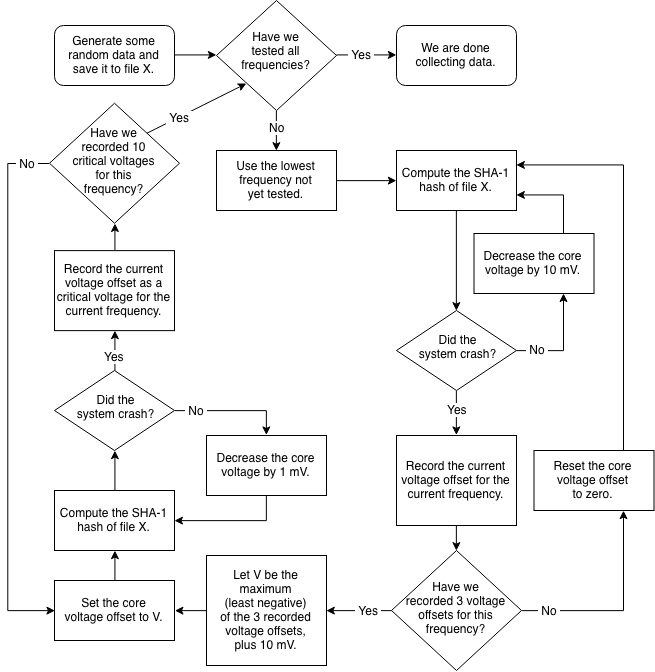
\includegraphics[width=\columnwidth,keepaspectratio]{data-collection-flowchart.png}}
    \caption{
        \label{fig:data-collection-flowchart}
        Flowchart describing how we collect data to determine the critical
        points.
    }
\end{figure}

In particular, we first find the critical point to the nearest 10 mV, performing
three (3) repetitions. We assume that the crticial point does not lie above the
maximum of these data points, plus another 10 mV for assurance. We then find the
critical point to as much accuracy as is possible (i.e. to the nearest 10 mV)
by testing every possible voltage offset within this narrower range, performing
ten (10) repetitions. We plot the mean, minimum, and maximum of these 10 data
points for each possible frequency in Figure \ref{fig:critical-points-graph}.
In this figure, the blue crosses are the mean voltage offset for each frequency.
The red diamonds are the bounds for the corrseponding error bars.

\begin{figure}[!htb]
    \center{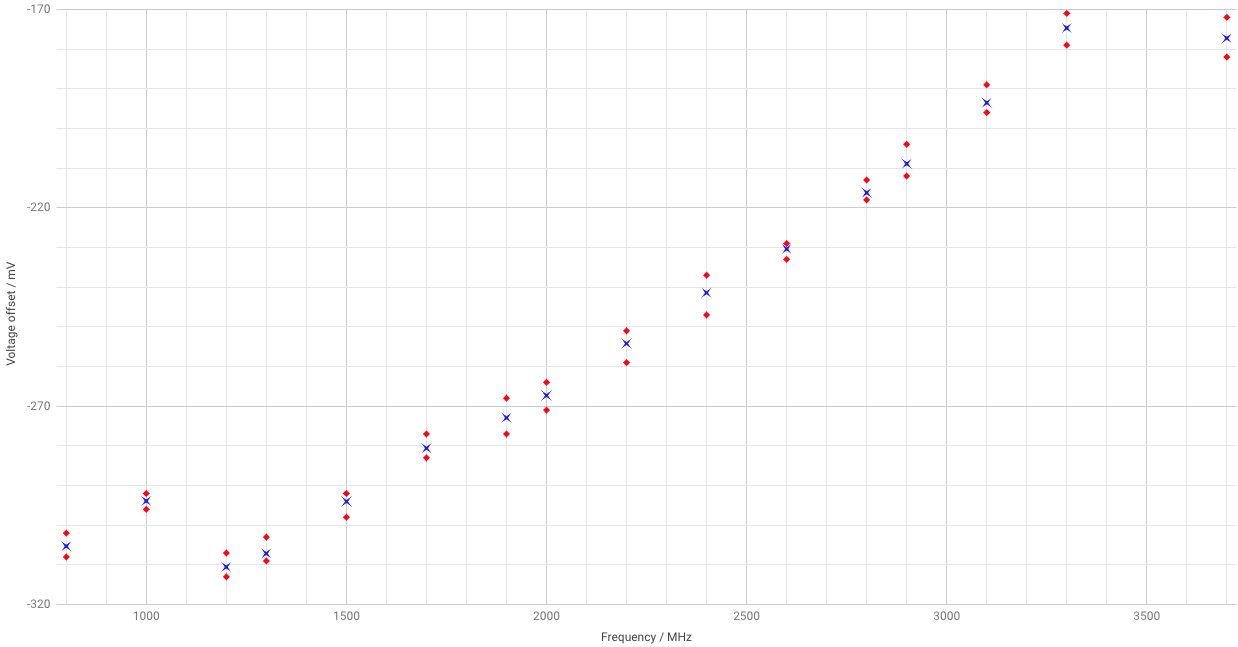
\includegraphics[width=\columnwidth,keepaspectratio]{critical-points-graph.png}}
    \caption{
        \label{fig:critical-points-graph}
        Graph plotting voltage offset against frequency for data points we have
        collected concerning critical points.
    }
\end{figure}

Ideally, this data collection would be automated, with the testbench running
through the process detailed above on boot, recording the tested OPPs to disk,
and rebooting after a system crash to repeat the process for different
frequencies as required. In practice, this is not possible, for the following
reasons:
\begin{itemize}
    \item any data that ought to be written to disk may not actually be flushed
        from memory to disk before the sytem encounters a kernel panic, 
        resulting in loss of these data; and
    \item the system does not always reboot after encountering a kernel panic,
        contrary to the operating system's intended function of rebooting 30
        seconds after a kernel panic. In such situations, the machine must be
        reset manually.
\end{itemize}

As such, we collect the data by hand with the aid of a shell script,
\code{undervolt-test.sh}, details of which are given in
§\ref{sec:undervolt-test.sh}.


\section{Demonstrating the viability of power management attacks}
\label{sec:observing-fault}

In order to demonstrate that a power management attack is possible on this
platform, we attempt to induce a computational fault whilst the SHA-1 hash of
some known data with a known hash is being computed. The aim is for the fault
to result in an incorrect hash being computed. The process is as follows:

\begin{enumerate}
    \item Choose a critical point.
    \item \label{item:stableOPP} Put the system into a stable OPP near the
        chosen critical point.
    \item \label{item:beginSHA} Begin computing the SHA-1 hash of the known data.
    \item \label{item:induceFault} Whilst the hash is being computed,
        \emph{briefly} put the system into an unstable OPP near the chosen
        critical point.
    \item The hash computation ends, and we hope to see an incorrect hash.
\end{enumerate}

We use the data collected in §\ref{sec:unstableOPPs} to choose a stable OPP and
an unstable OPP which both use the same frequency and lie near the
stable–unstable boundary line. The larger the error bars are near this dividing
line for a given frequency, the less clear the distinction between the stable and
unstable regions for that frequency. As such, since the data for 2600~MHz has
the smallest error bar, we will choose OPPs with a frequency of 2600~MHz.
The data we collected shows that the mean critical voltage for 2600~MHz
is $-230.4$~mV. Thus, we decide that the voltage offset of our stable OPP
should be greater than (i.e. more positive than) $-230.4$~mV, and that of the
unstable OPP should be less than (i.e. more negative than) $-230.4$~mV.

In order to perform steps \ref{item:stableOPP} and \ref{item:induceFault}, we
need the ability to alter the voltage scaling parameters of the CPU. Using the
\code{undervolt} utility discussed in §\ref{sec:undervolt} will not afford us the
timing precision required to execute step \ref{item:induceFault} briefly enough
to induce a fault without completely crashing the system. As such, we opt to
write our own program which will alter the voltage scaling paramters in a
suitably brief manner, which requires us to be able to write to the necessary
MSR as discussed in §\ref{sec:undervolt}. This is ultimately done via execution
of the \code{WRMSR} assembly instruction of the x86
architecture~\cite[Vol. 2, §4.4]{intelDevManual}. Since this instruction
must be executed at privilege level 0 or in real-address mode, we cannot
execute it from userspace; we need to do so in kernel mode. We therefore write
a custom kernel module to set the voltage offset at the necessary times.

We take the approach of simply demonstrating that successful fault injection is
possible, rather than developing a fully-formed attack on a program running in
userspace. That is, we could develop a malicious kernel module which lies in
wait until a hash computation begins in userspace, e.g. an
instance of GnuPG's \code{sha1sum} program begins running. Upon detecting that
such a program is running, the kernel module would have to correctly time the
execution of step \ref{item:induceFault} as discussed in~\cite[§3.5]{clkscrew}.
Instead, we take the less complex approach of adapting the source code of
\code{sha1sum}~\cite{gnupgSHA} into a kernel module which, when inserted into
the kernel, performs steps \ref{item:stableOPP}, \ref{item:beginSHA}, and
\ref{item:induceFault}, all in kernel mode. In this way, we can directly add
instructions to the \code{sha1sum} source code to alter the core voltage at
the necessary times. The details of the kernel module we developed for this
purpose, dubbed \code{bad\_sha}, are given in §\ref{sec:bad-sha}. We experiment
with the following parameters:

\begin{itemize}
    \item the voltage offset of the chosen stable OPP;
    \item the voltage offset of the chosen unstable OPP; and
    \item the amount of time in which the unstable OPP is used;
\end{itemize}
and we see that we can successfully induce a fault around $2\%$ of
the time when we use $-225$~mV for the stable OPP, $-234$~mV for the unstable
OPP, and the unstable OPP is in use whilst five (5) 32-bit W-blocks are processed
during the SHA-1 hash computation (where a W-block is defined as in~\cite[§6.1]{rfcSHA}).




\subsection{Tools}

